\documentclass{beamer}
\usepackage{bm}
\usepackage{graphicx}
%\graphicspath{ {./images/} }
\usetheme{Darmstadt}
\title{Dissipation and dispersion in finite difference solutions of hyperbolic PDEs}
\subtitle{Numerical solutions of PDEs}
\author{Gabriele Cimador}
\institute{Data Science and Scientific computing at Università di Trieste}
\date{\today}
\begin{document}
\begin{frame}
\titlepage
\end{frame}
\begin{frame}
\frametitle{Summary}
\tableofcontents
\end{frame}
\section{Hyperbolic problems}
\begin{frame}
Usually transport wave-like phenomena with finite speed of propagation. Examples:
\begin{itemize}
  \item 1d transport/advection eq. $u_t + a u_x = 0$
  \item Conservation laws $u_t + (f(u))_x = 0$
  \item Wave eq. $u_{tt} + cu_{xx} = 0$
\end{itemize}
\end{frame}
\begin{frame}
All of the prevoius can be grouped with the general tranport system of equations:
\begin{align*}
\bm{u}_t + A\bm{u}_x = 0
\end{align*}
where $A$ matrix which can depend on $t, x, \bm{u}$ and has a full set of real eigenvalues.
\\ e.g. for the conservation law equation
\begin{align*}
u_t + (f(u))_x = 0 \Rightarrow u_t + A(u)u_x = 0
\end{align*}
 where $A(u) = \frac{\partial f}{\partial u}$.
\end{frame}
\begin{frame}
\begin{itemize}
  \item There is no dissipation: $\lVert u(t,\cdot) \rVert_{L_2} = \lVert u_0\rVert_{L_2}$
  \item Information propagates at finite speed
  \item Discontinuites in initial data is propagated $\Rightarrow$ discontinue solution
  \item CFL condition necessary for convergence of a finite difference scheme
\end{itemize}
\end{frame}
\section{Finite differences}
\begin{frame}
\frametitle{Finite differences}
If the PDE is defined in a domain $I \times \Omega$ where $I$ is the time interval $[0, T_f]$ and $\Omega$ is the space domain of one variable $[a,b]$, we can discretize the PDE domain with $N_t \times N_x$ points. We can than define a general explicit difference scheme at time $t = t_n$ as
\begin{align*}
v_j^{n+1} = \sum_{i = -l}^r \beta_i v_{j+i}^n
\end{align*}
where $j = l, ..., N_x - r -1$, $n = 0, ..., N_t$ and $v_j^n$ is a mesh function over the discretised domain.
\end{frame}
\begin{frame}
If: \begin{itemize}
\item PDE has constant coefficients
\item Problem is defined on infinte mesh or has periodic boundary conditions
\end{itemize}
Can perform a Fourier analysis of how the difference scheme acts on the initial condition. \\ If $\hat{v}(t,\xi)$ is Fourier transform of the solution and $\iota = \sqrt{-1}$, we have
\begin{align*}
v(t,x) = \frac{1}{\sqrt{2\pi}}\int_{-\infty}^{\infty}e^{\iota\xi x}\hat{v}(t,\xi)d\xi
\end{align*}
\end{frame}
\begin{frame}
The difference scheme gives
\begin{align*}
\int_{-\infty}^{\infty}e^{\iota\xi x}\hat{v}(t + \tau,\xi)d\xi = & \sum_{i=-l}^{r}\beta_i\int_{-\infty}^{\infty}e^{\iota\xi (x + ih)}\hat{v}(t,\xi)d\xi \\
= & \int_{-\infty}^{\infty} \left(\sum_{i=-l}^{r}\beta_i e^{\iota\xi ih}\right) e^{\iota \xi x}\hat{v}(t,\xi)d\xi \\
\sum_{i=-l}^{r}\beta_i e^{\iota\xi ih} = g(\zeta) \ \Rightarrow & \ \hat{v}(t + \tau, \xi) = g(\zeta)\hat{v}(t,\xi)
\end{align*}
$\zeta = \xi h, \ \tau = \frac{T_f}{N_t}, \ h = \frac{b - a}{N_x}$
\end{frame}
\begin{frame}
$g(\zeta)$ is the \textbf{amplification factor} and $\hat{v}(t,\xi) = g(\zeta)^n\hat{v}(0,\xi)$
\begin{itemize}
\setlength\itemsep{1em}
\item $\|g\| \Rightarrow$ analysis of dissipation of wave numbers
\item $Arg(g) \Rightarrow$ analysis of dispersion of wave numbers
\item If the PDE has $s$ components than $g$ is an $s \times s$ \textbf{amplification matrix} $G$. Dissipation and dispersion studied via the eigenvalues of $G$.
\end{itemize}
Dissipation and dispersion in the finite difference scheme can occur even if the PDE has not these characteristics.
\end{frame}
\begin{frame}
\frametitle{Advection equation}
Consider the advection equation equipped with initial and boundary condition:
$$
\begin{cases}
u_t + a u_x = 0, & x,t \in [a,b] \times [0,T_f] \\
u(0,x) = u_0, & x \in [a,b]
\end{cases}
$$
Boundary condition depends on the sign of $a$. e.g. if $a > 0$ the boundary condition reads $u(a,t) = f(t) \ \forall \ t \ \in [0,T_f]$
\end{frame}
\section{Upwind method}
\begin{frame}
\frametitle{Upwind method}
Considering a discretization of $[0,T_f] \times [a,b]$ and that $U_j^n$ is mesh function approximating $u$ solution of PDE we can discretize the operators as follows:
\[
\begin{cases}
\displaystyle{\frac{U_j^{n+1} - U_j^n}{\tau} = \frac{U_j^n - U_{j-1}^n}{h}}, & \text{if } a > 0 \\ 
\\
\displaystyle{\frac{U_j^{n+1} - U_j^n}{\tau} = \frac{U_{j+1}^n - U_j^n}{h}}, & \text{if } a < 0
\end{cases}
\]
$n = 0, ..., N_t - 1$
\end{frame}
\begin{frame}
\frametitle{Upwind method}
Can be rewritten as:
\[
U_j^{n+1} =
\begin{cases}
(1 - \nu) U_j^n + \nu U_{j - 1}^n & \text{if } a > 0 \\
(1 + \nu) U_j^n - \nu U_{j + 1}^n & \text{if } a < 0
\end{cases}
\]
where $\nu = a \displaystyle{\frac{\tau}{h}}, \ n = 0, ..., N_t - 1$
\end{frame}
\begin{frame}
Amplification factor for $a > 0$ is $g(\zeta) = (1 - \nu) + \nu e^{-\iota \xi h}$:
\begin{itemize}
\setlength\itemsep{1em}
\item $ \|g\| \ \leq \ 1 \ \forall \ \xi \iff  0 \leq |\nu| \leq 1$
\item Dissipative scheme
\item Monotone scheme: if $\nu \leq 1 \ \Rightarrow \ \max_j{|v_j^{n+1}|} \leq \max_j{|v_j^n|}$
\\ $\Rightarrow$ stability even if $a = a(x,t) \iff |a_j^n \frac{\tau}{h}| \leq 1$
\item $Arg(g) = \displaystyle{-\tan^{-1}\left(\frac{\nu \sin{\xi h}}{(1 - \nu) + \nu \cos{\xi h}}\right)}$
\end{itemize}
\end{frame}
\begin{frame}
PDE admits plane-wave solutions of the form
\begin{align*}
u(t,x) = e^{\iota(\xi x + \omega t)}
\end{align*}
where $\xi = $ wave number, $\omega = $ frequency. \\
PDE imposes the \textbf{dispersion relation} $\omega = \omega(\xi)$ and \textbf{phase velocity} $c = \frac{\omega}{\xi}$. e.g. Advection eq. imposes $\omega = -a\xi$ and $c = -a$ independent on wave number. \\
To study dispersion, we can study the ratio $\phi_e = \frac{Arg(g)}{\omega}$
\end{frame}
\begin{frame}
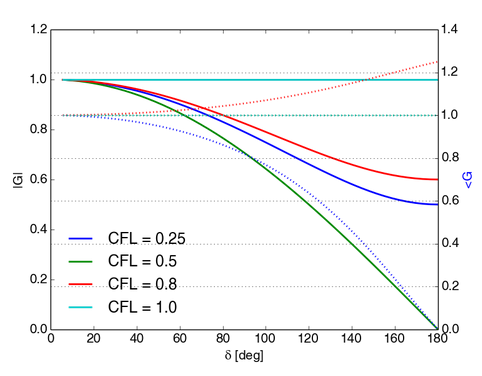
\includegraphics[width=\textwidth]{up_g}
\end{frame}
\begin{frame}
Dissipation can be explained also as follows:
\begin{align*}
0 \ = \ & \frac{U_j^{n+1} - U_j^n}{\tau} + a \frac{U_j^n - U_{j-1}^n}{h} = \\
= \ & \frac{U_j^{n+1} - U_j^n}{\tau} + a \frac{U_{j+1}^n - U_{j-1}^n}{2h} - \frac{a * h}{2}\frac{U_{j+1}^n -2U_j^n + U_{j-1}^n}{h^2}
\end{align*}
i.e. it is a difference scheme for the parabolic PDE
\begin{align*}
u_t + a u_x - \frac{a h}{2}u_{xx} = 0
\end{align*}
So upwind scheme pollutes PDE with artificial diffusion.
\end{frame}
\section{Lax-Wendroff}
\begin{frame}
\frametitle{Lax-Wendroff}
It takes the form
\begin{align*}
U_j^{n+1} = \frac{1}{2}\nu(1 + \nu)U_{j-1}^n + (1 - \nu^2)U_j^n - \frac{1}{2}\nu(1 - \nu)U_{j+1}^n
\end{align*}
Can be rewritten as 
\begin{align*}
\frac{U_i^{n+1} - U_i^n}{\tau} + a \frac{U_{i+1}^n - U_{i-1}^n}{2h} - \frac{\tau a^2}{2}\frac{U_{i+1}^n -2U_i^n + U_{i-1}^n}{h^2} = 0
\end{align*}
So it approximates the PDE $u_t + au_x = \frac{\tau a^2}{2}u_{xx}$. Comparing with upwind:
\begin{align*}
\frac{|a|}{2} = \frac{|a|\tau}{2 \nu} = \frac{a^2 \tau}{2 |a| \nu} \geq \frac{a^2 \tau}{2}
\end{align*}
So LW expected to be less dissipative.
\end{frame}
\begin{frame}
Amplification factor
\begin{align*}
g(\zeta) = 1 - 2 \eta^2\sin^2{\frac{1}{2}\zeta} - \iota \eta \sin{\zeta}
\end{align*}
\begin{itemize}
\setlength\itemsep{1em}
\item $|g|^2 = 1 - 4\nu^2(1-\nu^2)\sin^4{\frac{1}{2}\zeta} \ \leq 1 \iff |\nu| \leq 1$ \\ Order of amplitude error $\zeta^4$ when $\zeta = h\xi$ small
\item $Arg(g) = \displaystyle{-\tan^{-1}{\frac{\nu \sin{\zeta}}{1 - 2\nu^2\sin^2{\frac{1}{2}\zeta}}}}$
\end{itemize}
\end{frame}
\begin{frame}
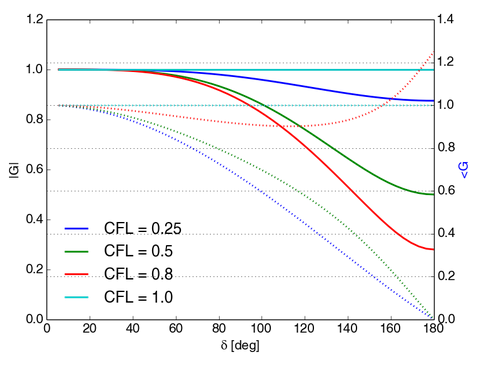
\includegraphics[width=\textwidth]{lw_g}
\end{frame}
\begin{frame}
\frametitle{Lax-Wendroff with variable coefficient}
Now $a = a(x,t)$
\end{frame}
\section{Leap-frog}
\begin{frame}
\frametitle{Leap-frog scheme}
\begin{align*}
\frac{U_j^{n+1} - U_j^{n-1}}{2\tau} + a \frac{U_{j+1}^n-U_{j-1}^n}{2h} = 0
\end{align*}
\textit{Oss.:} need special procedure to obtain $U_1$, e.g. with Lax-Wendroff \\
\end{frame}
\begin{frame}
Fourier analysis gives
\begin{align*}
g(\zeta) = -\iota\nu\sin{\zeta} \pm \sqrt{1 - \nu^2\sin^2{\zeta}}
\end{align*}
\begin{itemize}
\setlength\itemsep{1em}
\item $|g|^2 = 1 \iff \nu \leq 1 \ \Rightarrow$ no dissipation
\item Presence of two solutions $\Rightarrow$ spurious solution mode
\end{itemize}
\end{frame}
\section{Box method}
\begin{frame}
\frametitle{A finite volume scheme - Box method}
Suppose conservation law $u_t + f(u)_x = 0$ and integrate it over a region $\Omega = [t_n,t_{n+1}] \times [x_j,x_{j+1}]$. Gauss divercence theorem gives
\begin{align*}
\iint_\Omega(u_t + f_x)dxdt & \equiv \iint_\Omega div(f,u)dxdt \\
& = \oint_{\partial\Omega}[fdt-udx]
\end{align*}
\end{frame}
\begin{frame}
Approximating the integral with the trapezoidal rule gives the box method:
\begin{align*}
\frac{U_{j+1}^{n+1} + U_j^{n+1} - U_{j + 1}^n - U_j^n}{2\tau} + \frac{F_{j+1}^{n+1} + F_{j+1}^n - F_j^{n+1} - F_j^n}{2h} = 0
\end{align*}
For the advection equation $f = au$ and the method becomes:
\begin{align*}
U_{j+1}^{n+1} = U_j^n + (1 + \nu)^{-1}(1 - \nu)(U_{j+1}^n - U_j^{n+1})
\end{align*}
where  $\nu =  a\frac{\tau}{h}$
\end{frame}
\begin{frame}
Amplification factor $g(\zeta) = \frac{\cos{\frac{1}{2}\zeta} - \iota\nu\sin{\frac{1}{2}\zeta}}{\cos{\frac{1}{2}\zeta} + \iota\nu\sin{\frac{1}{2}\zeta}}$:
\begin{itemize}
\setlength\itemsep{1em}
\item $|g| = 1 \ \forall \ \nu \ \Rightarrow$ unconditionally stable, no dissipation
\item $Arg(g) = -2\tan^{-1}{\nu\tan{\frac{1}{2}\zeta}}$
\end{itemize}
\end{frame}
\begin{frame}
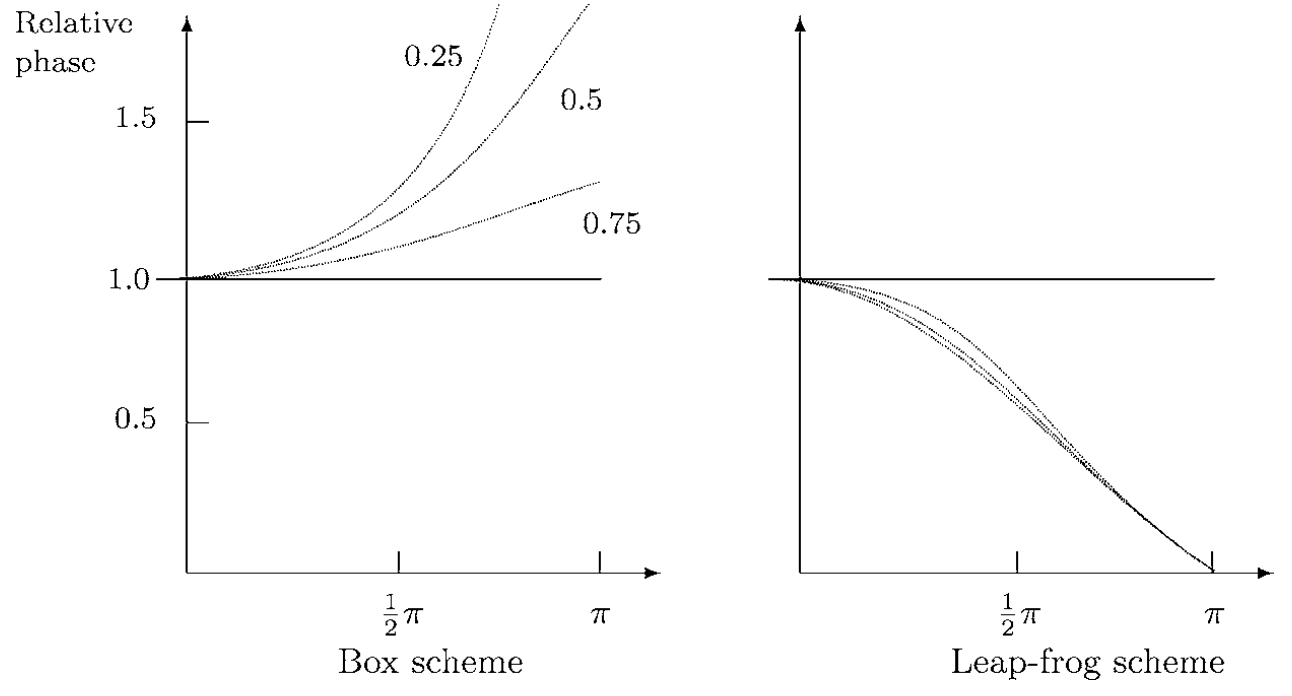
\includegraphics[width=\textwidth]{lp_bx_lag}
\end{frame}
\begin{frame}
conservation law - burgers
\end{frame}
\begin{frame}
bibliography
\end{frame}
\end{document}
